\section{Results}
\label{sec:results}

We organize our results around three questions: (1) Can \llms distinguish epistemic from non-epistemic beliefs? (2) How does the decodability of truth value compare to opinion agreement? (3) How do these patterns change with model scale?

\subsection{Type Classification: Epistemic vs.\ Non-Epistemic}
\label{sec:type_results}

\para{Near-perfect classification from middle layers onward.}
All four GPT-2 models achieve near-perfect accuracy at distinguishing epistemic from non-epistemic statements. \tabref{tab:type_results} shows that peak type classification accuracy ranges from 99.2\% (\gptsmall) to 100\% (\gptmedium and \gptlarge). Even the smallest model (117M parameters) reaches 99.2\% by layer 8 (normalized depth 0.67). All models exceed 90\% accuracy from approximately layer 3 onward, suggesting that the epistemic/non-epistemic distinction is encoded early and robustly.

\para{High selectivity confirms genuine encoding.}
The selectivity scores for type classification are 0.485 (\gptsmall) and 0.448 (\gptxl), with random-label control probes achieving only 50.6--50.8\% accuracy. This large gap confirms that the near-perfect type classification reflects genuine representational structure rather than probe memorization.

\begin{table}[t]
\centering
\caption{Non-epistemic agreement probing and type classification results. Peak accuracy and corresponding layer are shown. Selectivity is the gap between true-label and random-label accuracy. Best results per column in \textbf{bold}.}
\begin{tabular}{@{}lccccc@{}}
\toprule
\textbf{Model} & \textbf{Non-Epist.\ Acc.} & \textbf{Peak Layer} & \textbf{Type Acc.} & \textbf{Peak Layer} & \textbf{Selectivity} \\
\midrule
\gptsmall  & 86.7\% & L8  & 99.2\% & L8  & 0.485 \\
\gptmedium & 90.8\% & L12 & \textbf{100.0\%} & L14 & --- \\
\gptlarge  & \textbf{95.0\%} & L19 & \textbf{100.0\%} & L21 & --- \\
\gptxl     & 94.2\% & L26 & 99.6\% & L24 & 0.448 \\
\bottomrule
\end{tabular}
\label{tab:type_results}
\end{table}

\subsection{Epistemic Truth Probing}
\label{sec:truth_results}

\para{Domain-specific truth is moderately decodable.}
\tabref{tab:epistemic_results} presents peak mass-mean probing accuracy for epistemic truth across all models and domains. Within individual domains, accuracy ranges from 60.5\% (\companies, \gptmedium) to 88.5\% (\largerthan, \gptmedium). Geographic facts (\cities) show the strongest scaling trend, rising from 69.5\% in \gptsmall to 85.5\% in \gptxl. Numerical comparisons (\largerthan) achieve high accuracy across all scales.

\para{Cross-domain truth probing remains near chance.}
When all five epistemic domains are combined, peak accuracy drops to 53.5--59.0\%. This indicates that the mass-mean direction for truth is largely domain-specific: a ``truth direction'' learned from geographic facts does not generalize well to translation correctness or corporate facts.

\begin{table}[t]
\centering
\caption{Peak epistemic truth probing accuracy (\%) by dataset and model. Peak layer shown in parentheses. Best result per domain in \textbf{bold}.}
\resizebox{\textwidth}{!}{%
\begin{tabular}{@{}lccccc@{}}
\toprule
\textbf{Model} & \textsc{Cities} & \textsc{CommonClaims} & \textsc{Companies} & \textsc{LargerThan} & \textsc{All Combined} \\
\midrule
\gptsmall  & 69.5 (L9)  & 65.0 (L9)  & 61.5 (L5)  & 80.5 (L5)  & 53.5 (L5) \\
\gptmedium & 82.5 (L15) & 69.0 (L21) & 60.5 (L5)  & \textbf{88.5} (L9)  & 56.4 (L11) \\
\gptlarge  & 83.5 (L22) & \textbf{68.5} (L19) & \textbf{63.0} (L16) & 86.5 (L16) & 54.8 (L22) \\
\gptxl     & \textbf{85.5} (L22) & 67.5 (L21) & 61.5 (L15) & 86.0 (L3)  & \textbf{59.0} (L40) \\
\bottomrule
\end{tabular}
}
\label{tab:epistemic_results}
\end{table}

\subsection{Non-Epistemic Beliefs Are More Linearly Decodable Than Truth}
\label{sec:comparison}

\para{Opinion agreement outperforms truth probing.}
Across all models, non-epistemic agreement probing (86.7--95.0\%) substantially outperforms epistemic truth probing on the combined dataset (53.5--59.0\%). Even the best single-domain epistemic probe (\cities at 85.5\% for \gptxl) is comparable to or below non-epistemic probing for larger models.

\para{Statistical significance.}
\tabref{tab:statistical} reports paired $t$-tests comparing the full layer-wise accuracy profiles between epistemic (all combined) and non-epistemic probing. All four models show highly significant differences ($p < 10^{-7}$) with large effect sizes (Cohen's $d$ ranging from $-1.96$ to $-4.23$), confirming that non-epistemic beliefs are systematically more linearly decodable than epistemic truth.

\begin{table}[h]
\centering
\caption{Statistical comparison of layer-wise accuracy profiles between epistemic truth (all combined) and non-epistemic agreement probing. All differences are significant with large effect sizes.}
\begin{tabular}{@{}lcccc@{}}
\toprule
\textbf{Model} & \textbf{$t$-statistic} & \textbf{$p$-value} & \textbf{Cohen's $d$} & \textbf{Peak Layer Diff} \\
\midrule
\gptsmall  & $-18.46$ & $1.4 \times 10^{-13}$ & $-4.23$ & $-0.25$ \\
\gptmedium & $-15.16$ & $4.6 \times 10^{-12}$ & $-3.48$ & $-0.04$ \\
\gptlarge  & $-18.31$ & $1.6 \times 10^{-13}$ & $-4.20$ & $+0.08$ \\
\gptxl     & $-8.55$  & $6.2 \times 10^{-8}$  & $-1.96$ & $+0.29$ \\
\bottomrule
\end{tabular}
\label{tab:statistical}
\end{table}

\subsection{Layer-wise Patterns Across Model Scales}
\label{sec:layerwise}

\Figref{fig:cross_model} shows the normalized layer-wise probing accuracy for all three experiment types across the four GPT-2 models. Several patterns emerge.

\para{Type classification peaks consistently in middle layers.}
Across all models, type classification reaches near-ceiling accuracy by normalized depth 0.25--0.33 and peaks at 0.50--0.67. This consistency suggests that the epistemic/non-epistemic distinction is a fundamental organizational property of the representation space.

\para{Peak layers shift with model scale.}
For \gptsmall, epistemic truth peaks at normalized layer $\sim$0.42, while for \gptxl it peaks at $\sim$0.83. Non-epistemic agreement peaks at $\sim$0.67 for \gptsmall and $\sim$0.54 for \gptxl. This suggests that larger models require more layers to process factual information, while opinion processing stabilizes in middle layers regardless of scale.

\para{Epistemic truth accuracy scales with model size.}
On the combined epistemic dataset, peak accuracy increases from 53.5\% (\gptsmall, 117M) to 59.0\% (\gptxl, 1.5B). Domain-specific probing shows stronger scaling: \cities accuracy rises from 69.5\% to 85.5\%. This is consistent with the finding of \citet{marks2023geometry} that truth structure ``emerges with scale.''

\begin{figure}[t]
\centering
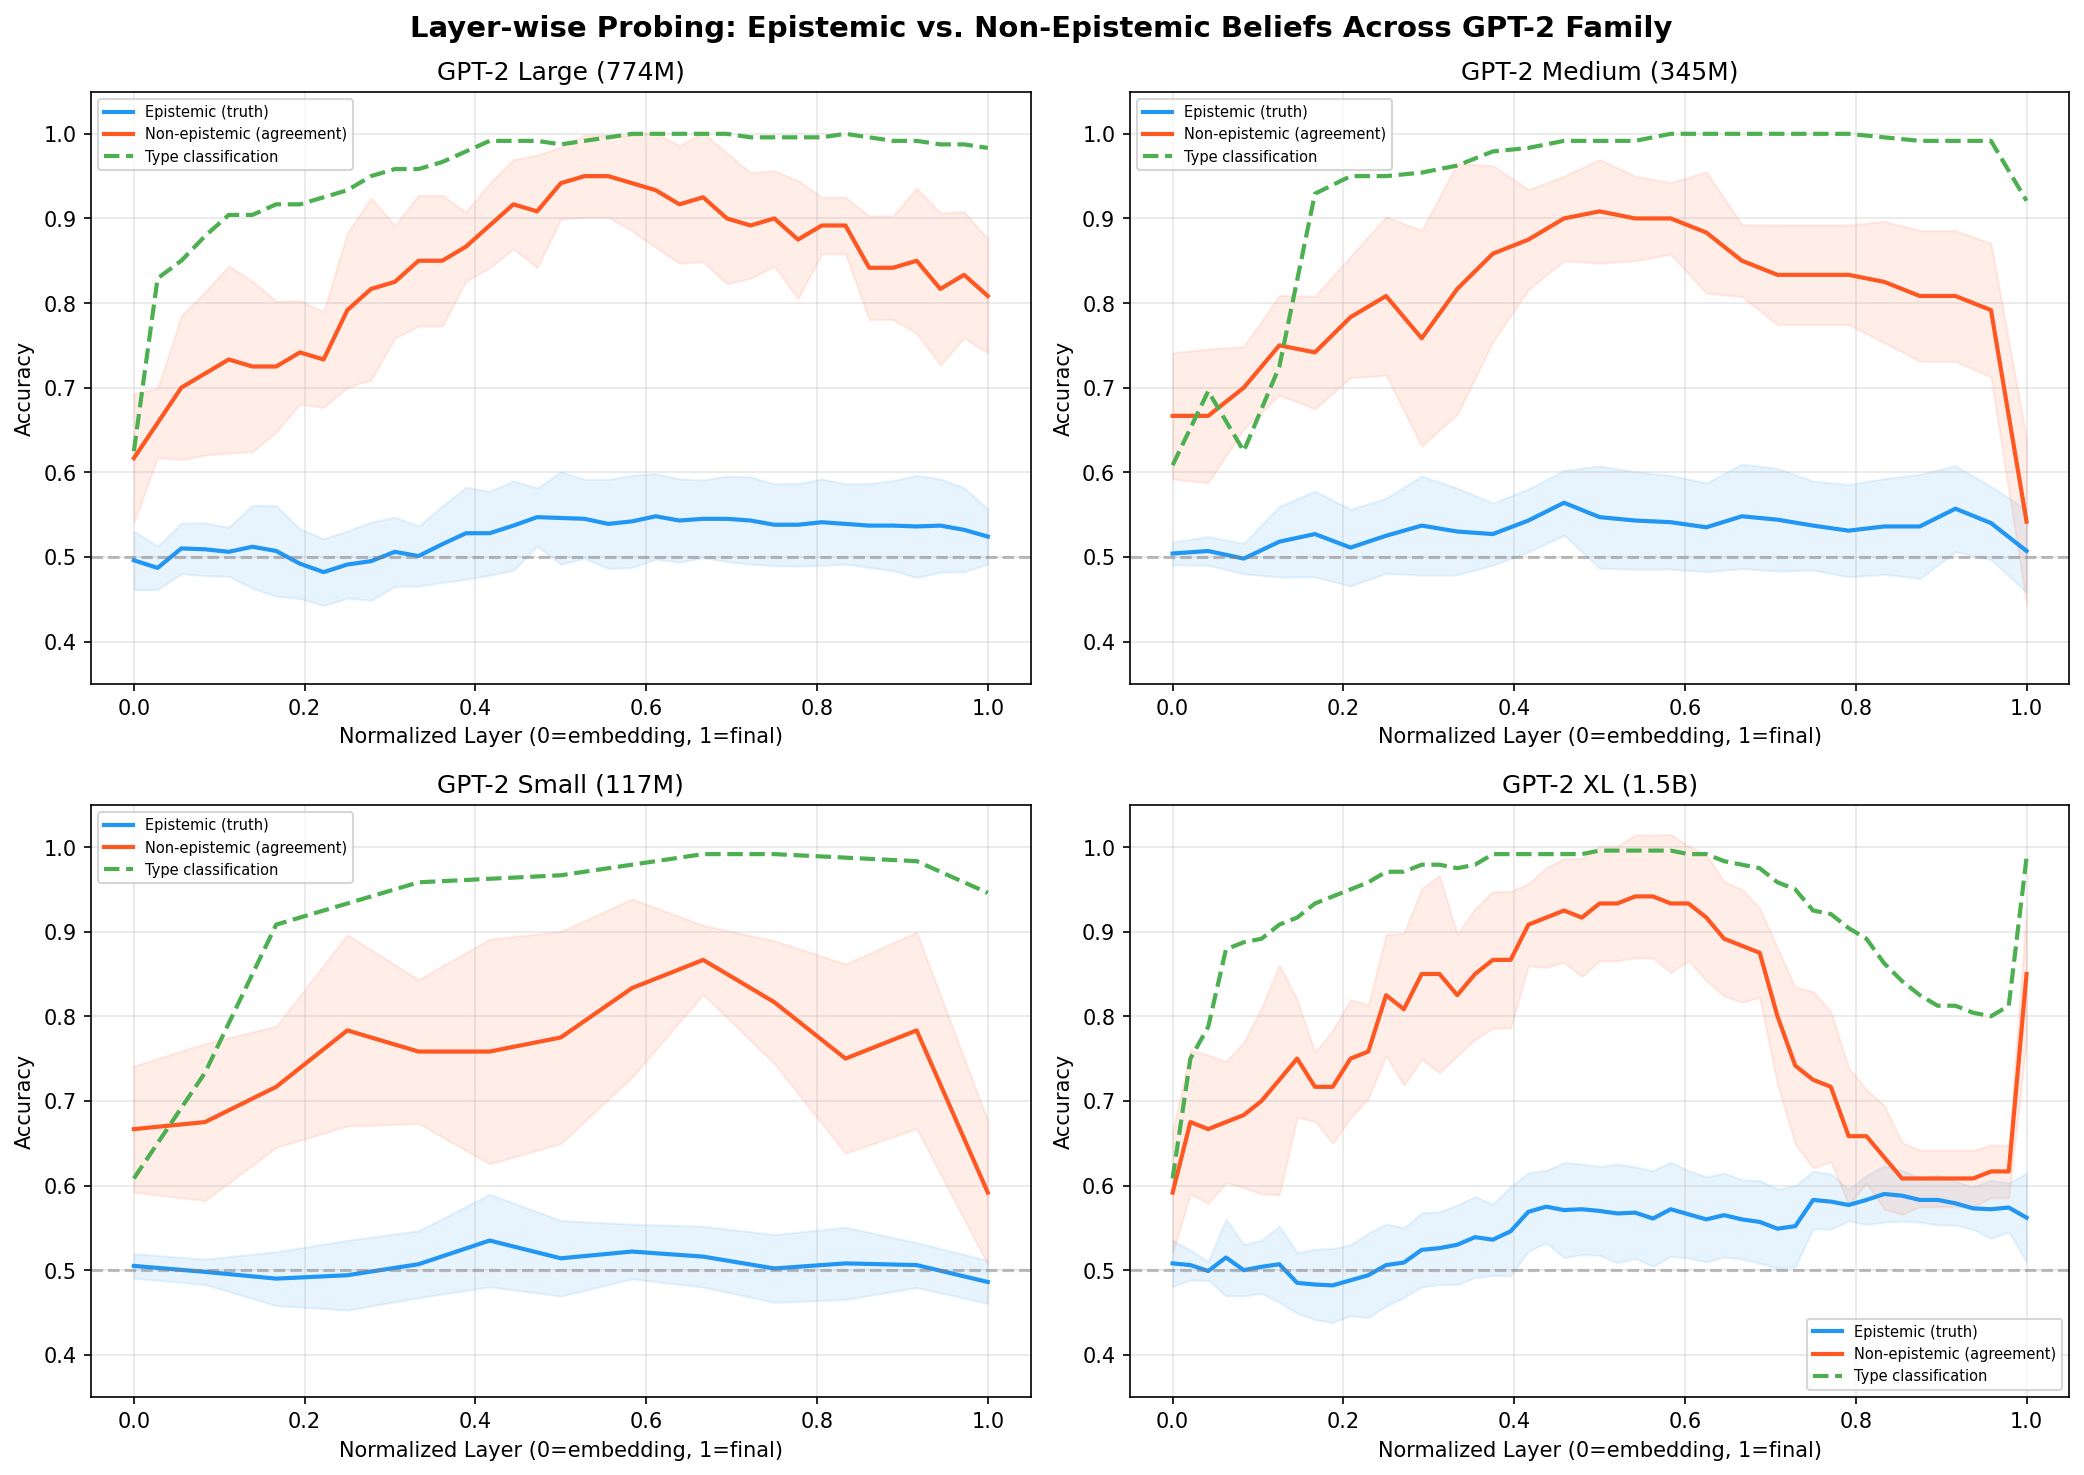
\includegraphics[width=0.95\linewidth]{figures/cross_model_comparison.png}
\caption{Normalized layer-wise probing accuracy across all four GPT-2 models for three experiment types: epistemic truth (combined dataset), non-epistemic agreement, and type classification (epistemic vs.\ non-epistemic). Layer indices are normalized to $[0, 1]$ for cross-model comparison. Type classification reaches near-perfect accuracy by normalized depth 0.25, while epistemic truth probing remains substantially lower than non-epistemic agreement across all depths and scales.}
\label{fig:cross_model}
\end{figure}

\subsection{Control and Transfer Analysis}
\label{sec:controls}

\para{Selectivity analysis.}
\Figref{fig:selectivity} shows the selectivity scores (true accuracy minus random-label control accuracy) across layers. For type classification, selectivity remains high (0.40--0.49) from middle layers onward, confirming that the near-perfect accuracy reflects genuine representational structure. For epistemic truth probing, selectivity is lower but still positive (0.03--0.09), consistent with the modest probing accuracy.

\para{Cross-dataset transfer.}
We train the mass-mean direction on one epistemic domain and evaluate on others. Transfer accuracy is generally above chance but lower than within-domain accuracy, indicating that truth representations are partially domain-specific. The \cities and \largerthan domains transfer best to each other, while \translations shows poor transfer, consistent with its low within-domain probing accuracy.

\begin{figure}[t]
\centering
\begin{subfigure}[b]{0.48\textwidth}
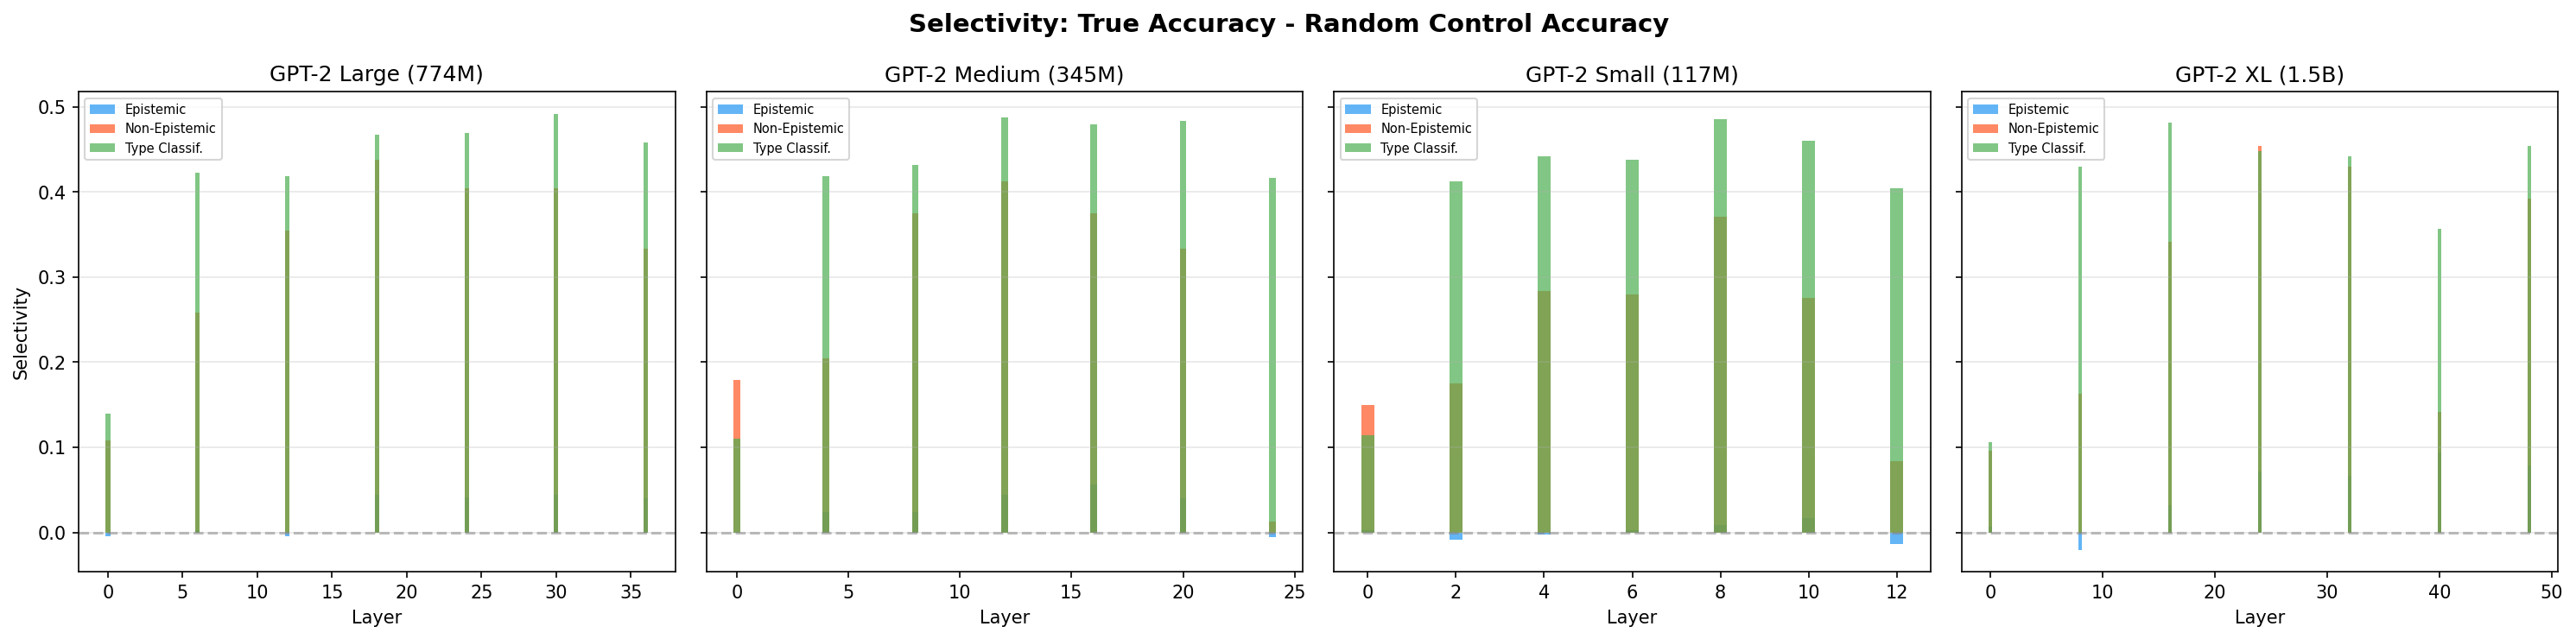
\includegraphics[width=\textwidth]{figures/selectivity.png}
\caption{Selectivity scores}
\label{fig:selectivity}
\end{subfigure}
\hfill
\begin{subfigure}[b]{0.48\textwidth}
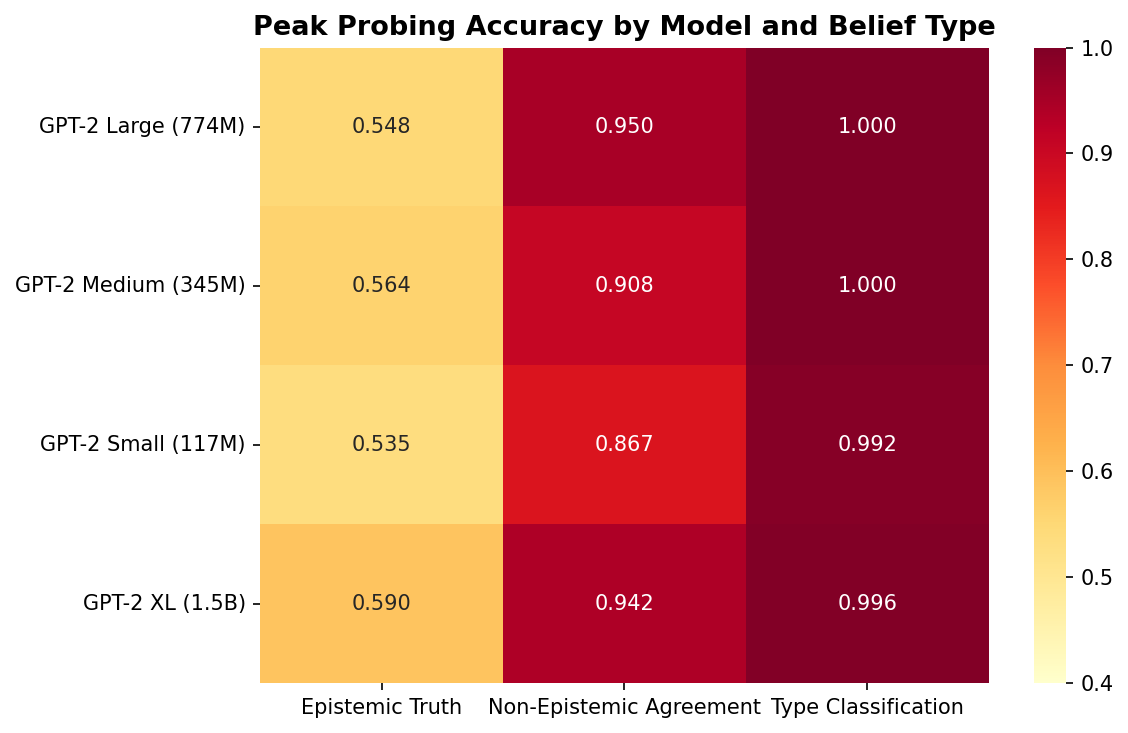
\includegraphics[width=\textwidth]{figures/summary_heatmap.png}
\caption{Peak accuracy heatmap}
\label{fig:heatmap}
\end{subfigure}
\caption{\captiona Selectivity scores (true accuracy minus random-label control) across layers for \gptsmall. High selectivity for type classification confirms genuine encoding. \captionb Peak probing accuracy across all models and experiment types. Non-epistemic and type classification consistently outperform epistemic truth probing.}
\label{fig:controls}
\end{figure}
